%% ID: chain_on_peg
%% TITLE: A Chain on a Peg
%% TYPE: question
%% QUESTIONTYPE: symbolic
%% CONCEPTS: energy
%% VIDEOS: 
%% LEVEL: 5
%% TOPIC: mechanics/dynamics
%% ORDER: 9


\begin{problem}[HSC1932AMQ7l] % somewhat hard      but interesting...
 {A heavy uniform chain hangs over a small smooth peg with equal lengths \vari{a} on each side.  Masses \vari{m} and \vari{3m} are attached to the two ends, and the system is released from rest.  Prove, by the principle of conservation of energy, that the mass \vari{m} reaches the peg with velocity \vari{\sqrt{ga}}, whatever the mass of the chain may be.}
{\stress{Used with permission from UCLES, Higher School Certificate Applied Mathematics, June 1932, Question 7.}}
{Drawing a diagram of the system at the two points of interest is a key first step, as in Figure \ref{fig:Dynamics_chain_pulley}.

\begin{figure}[h]
  \centering
 	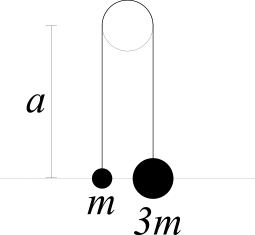
\includegraphics[width=0.4\linewidth]{../../../figures/Dynamics_chain_pulley_1.svg}
	\caption{}\label{fig:Dynamics_chain_pulley_1}
\end{figure}
\begin{figure}{0.5\textwidth}
	\centering
	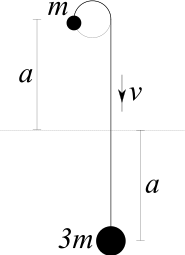
\includegraphics[width=0.4\linewidth]{../../../figures/Dynamics_chain_pulley_2.svg}
	\caption{}\label{fig:Dynamics_chain_pulley_2}
\end{figure}

There are only two forms of energy that come into play; kinetic energy and gravitational potential energy. In order to use the gravitational potential energy, we need to define a position for the zero. The equations will be simplest if the zero is level with the masses initially; the dotted line in the diagrams. Initially the only energy is the potential energy of the hanging chain, which we will find in the general way by integrating the potential of small elements, \vari{\d m}, of the chain. In order to complete the integration we need \vari{\d m} in terms of \vari{\d h}, the height element; \valuedef{\d m}{\lambda \d h}{}, where \vari{\lambda} is the mass per unit length of the chain. There are two sections of chain hanging, going from \vari{0} to \vari{a} in height:
\begin{eqnarray*} 
\text{Initial Energy} &= 2 \int gh \d m \\ 
&= 2 \int_{0}^{a} gh \lambda \d h \\ 
&= 2\lambda g\left[\frac{1}{2}h^{2}\right]_{0}^{a} \\ 
&= \lambda ga^{2} 
\end{eqnarray*}
and this result could have been found by considering the two sections of chains to have mass \vari{a\lambda} acting at the height of the centre of mass, \vari{\frac{a}{2}}.

When the mass \vari{m} reaches the peg there are the kinetic energies of the two masses and the chain, and the gravitational potential energies of all three, to take into account. This time the chain stretches from \vari{-a} to \vari{a}, and so these will form the new limits of integration. The total mass of the chain is \vari{2a\lambda} and it all moves at a speed vari{v}:
\begin{eqnarray*} 
\text{Final Energy} &= \frac{1}{2}(m)v^{2} + \frac{1}{2}(3m)v^{2} + \frac{1}{2}(2a\lambda)v^{2} + \int_{-a}^{a}gh\lambda \d h + (m)(g)(a) + (3m)(g)(-a) \\
			&= 2mv^{2} + a\lambda v^{2} + g\lambda\left[\frac{1}{2}h^{2}\right]_{-a}^{a} - 2mga \\ &= 2mv^{2} + a\lambda v^{2} - 2mga \\ 
			&= (2m + \lambda a)v^{2} - 2mga 
\end{eqnarray*}
where the potential energy of the chain is zero because its mass is symmetrically distributed about the zero of our scale.

Then conservation of energy gives:
\begin{eqnarray*} 
\text{Final Energy} &= \text{Initial Energy} \\ 
(2m + \lambda a)v^{2} - 2mga &= \lambda ga^2 \\ 
(2m + \lambda a)v^{2} &= 2mga + \lambda ga^{2} \\
	v^{2} &= \frac{ga(2m + \lambda a)}{2m + \lambda a} \\
	 &= ga \\ 
	 v &= \sqrt{ga} 
\end{eqnarray*}
as required.
}
\end{problem}